\section{Auswertung}
\label{sec:Auswertung}

\subsection{Bestimmung der Winkelrichtgröße}

Die Messung wird mit einem senkrechten Abstand von ${r=\SI{4.0}{\centi\meter}}$ durchgeführt. 
Der Auslenkwinkel $\varphi$ und die aufgewendete Kraft $F$ sind in \ref{tab:richtgrD} dargestellt, ebenso wie die sich daraus 
ergebenden Werte für die Winkelrichtgröße $D$. 
Sie berechnet sich, wie aus der Theorie zu entnehmen ist, über 
\begin{equation}
    D=\frac{Fr}{\varphi}\:.
\end{equation}

\begin{table}
    \centering
    \caption{Messwerte zur Bestimmung der Winkelrichtgröße.}
    \label{tab:richtgrD}
    \begin{tabular}{c S[table-format=1.2] S[table-format=1.2] S[table-format=2.1]}
        \toprule
        {$\varphi$} & {$\varphi\:/\:\symup{\pi}$} & {$F\:/\:\si{\newton}$} & {$D\:/\:\SI{e-3}{\newton\meter}$} \\
        \midrule
        \ang{26;;}  & 0.14  & 0.19 & 17.3 \\
        \ang{30;;}  & 0.17  & 0.21 & 15.7 \\
        \ang{37;;}  & 0.21  & 0.29 & 17.6 \\
        \ang{45;;}  & 0.25  & 0.41 & 20.9 \\
        \ang{60;;}  & 0.33  & 0.49 & 18.9 \\
        \ang{70;;}  & 0.39  & 0.61 & 19.9 \\
        \ang{81;;}  & 0.45  & 0.70 & 19.8 \\
        \ang{93;;}  & 0.52  & 0.74 & 18.1 \\
        \ang{100;;} & 0.56  & 0.91 & 20.7 \\
        \ang{110;;} & 0.61  & 0.97 & 20.2 \\
        \bottomrule
    \end{tabular}
\end{table}

Somit ergibt sich als experimenteller Wert ${D=\SI{18.9\pm1.6e-3}{\newton\meter}}$ für die Winkelrichtgröße. 
Die Abweichung der Größe berechnet sich über 
\begin{equation}
    \increment D = \sqrt{\frac{1}{N-1}\sum_{i=1}^N (D_i-\bar{D})^2}
    \label{eqn:fehler}
\end{equation}
mit dem arithmetischen Mittel $\bar{D}$. 

\FloatBarrier
\subsection{Bestimmung des Eigenträgheitsmoments der Drillachse}

Im Folgenden sei die Annahme eines nahezu masselosen Stabs, an dem zwei Punktmassen -- demnach ohne Ausdehnung -- 
gleicher Masse ${m=\SI{222.89}{\gram}}$ 
befestigt sind. 
In \ref{tab:I_D} sind die Messwerte entsprechend dargestellt. 
Es besteht ein linearer Zusammenhang zwischen den Quadraten der Periode $T$ und dem Abstand $a$ der Massen:

\begin{equation}
    T^2=\frac{4\symup{\pi}^2}{D}\bigl(I_\text{D} + m(a_1^2+a_2^2)\bigr)=:\frac{4\symup{\pi}^2}{D}(I_\text{D}+ma^2)    
    \label{eqn:Thoch2}
\end{equation} 

\begin{table}
    \centering
    \caption{Messwerte zur Bestimmung des Eigenträgheitsmoments $I_\text{D}$.}
    \label{tab:I_D}
    \begin{tabular}{S[table-format=2.1] S[table-format=2.1] S[table-format=4.1] S[table-format=1.2] S[table-format=2.2]}
        \toprule
        {$a_1\:/\:\si{\centi\meter}$} & {$a_2\:/\:\si{\centi\meter}$} & {$(a_1^2+a_2^2)\:/\:\si{\centi\meter\squared}$} & {$T\:/\:\si{\second}$} & {$T^2\:/\:\si{\second\squared}$} \\
        \midrule
        4.5  & 5.5  &   50.5 & 2.50 & 6.25  \\
        6.5  & 7.5  &   98.5 & 2.93 & 8.58  \\
        8.5  & 9.5  &  162.5 & 3.21 & 10.30 \\
        10.5 & 11.5 &  242.5 & 3.83 & 14.67 \\
        12.5 & 13.5 &  338.5 & 4.16 & 17.31 \\
        14.5 & 15.5 &  450.5 & 4.70 & 22.09 \\
        16.5 & 17.5 &  578.5 & 5.27 & 27.77 \\
        18.5 & 19.5 &  722.5 & 5.79 & 33.52 \\
        20.5 & 21.5 &  882.5 & 6.27 & 39.31 \\
        22.5 & 23.5 & 1058.5 & 6.78 & 45.97 \\
        \bottomrule
    \end{tabular}
\end{table}

Nun werden diese Werte in einem Diagramm aufgetragen. 
Mithilfe linearer Regression lässt sich aus dem Y-Achsenabschnitt $b$ der Eigenträgheitsmoment $I_D$ bestimmen. 
Die Steigung $c$ ergibt sich unter Vergleich mit \eqref{eqn:Thoch2} aus

\begin{gather}
y=b+cx \\
T^2 = \frac{4\symup{\pi}^2}{D}(I_\text{D}+ma^2) \\
\Rightarrow y = T^2, 
\quad b =  \frac{4\symup{\pi}^2}{D} I_\text{D}, 
\quad c = \frac{4\symup{\pi}^2}{D}m ,
\quad x = a^2 
\end{gather}

Unter Zuhilfenahme von \textit{Python 3.7.3} wird die lineare Regression durchgeführt, wie in Abbildung \ref{fig:Thoch2} zu sehen ist, und es ergibt sich der y-Achsenabschnitt~${b=\SI{4.42(25)}{\second\squared}}$
und eine Steigung von ${c=\SI{396.0\pm4.4}{\kilo\gram\per\joule}}$. 
Daraus lässt sich das Eigenträgheitsmoment zu 
\begin{equation}
    I_\text{D}=\frac{D}{4\symup{\pi}^2}b=\frac{m}{c}b=\SI{2.49(14)e-3}{\kilo\gram\meter\squared}
\end{equation}
bestimmen.

\begin{figure}
    \centering
    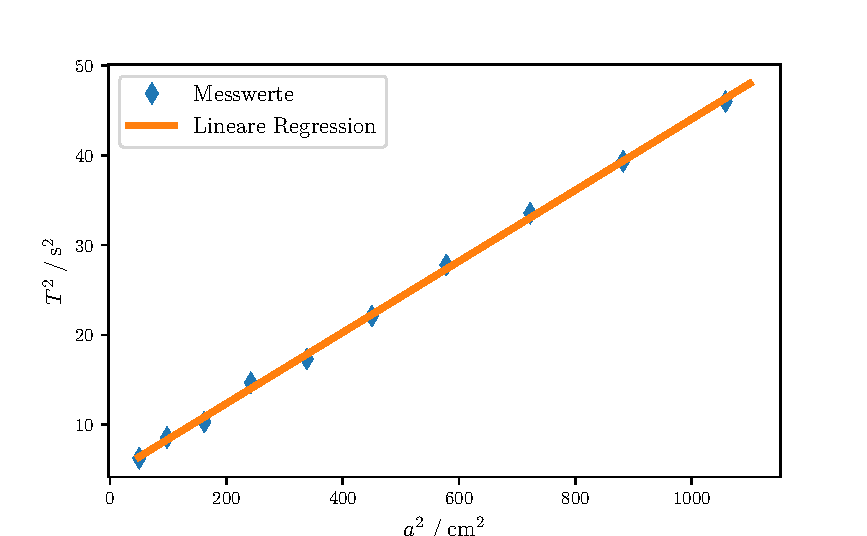
\includegraphics[width=0.8\textwidth]{plots/plot_I_D.pdf}
    \caption{Lineare Regression zur Bestimmung des Eigenträgheitsmoments.}
    \label{fig:Thoch2}
\end{figure}

\FloatBarrier
\subsection{Trägheitsmomente verschiedener Körper}

In den Tabellen \ref{tab:messSchwing} und \ref{tab:mittelSchwing} sind die Messwerte aufgetragen, die zur Bestimmung der 
Trägheitsmomente zweier verschiedener Zylinder und einer Holzpuppe in zwei unterschiedlichen Posen aufgenommen worden sind. 
In \ref{tab:mittelSchwing} berechnet sich der Messfehler ebenfalls über \eqref{eqn:fehler}. 

\begin{figure}
    \centering
    \begin{subfigure}{0.48\textwidth}
        \centering
        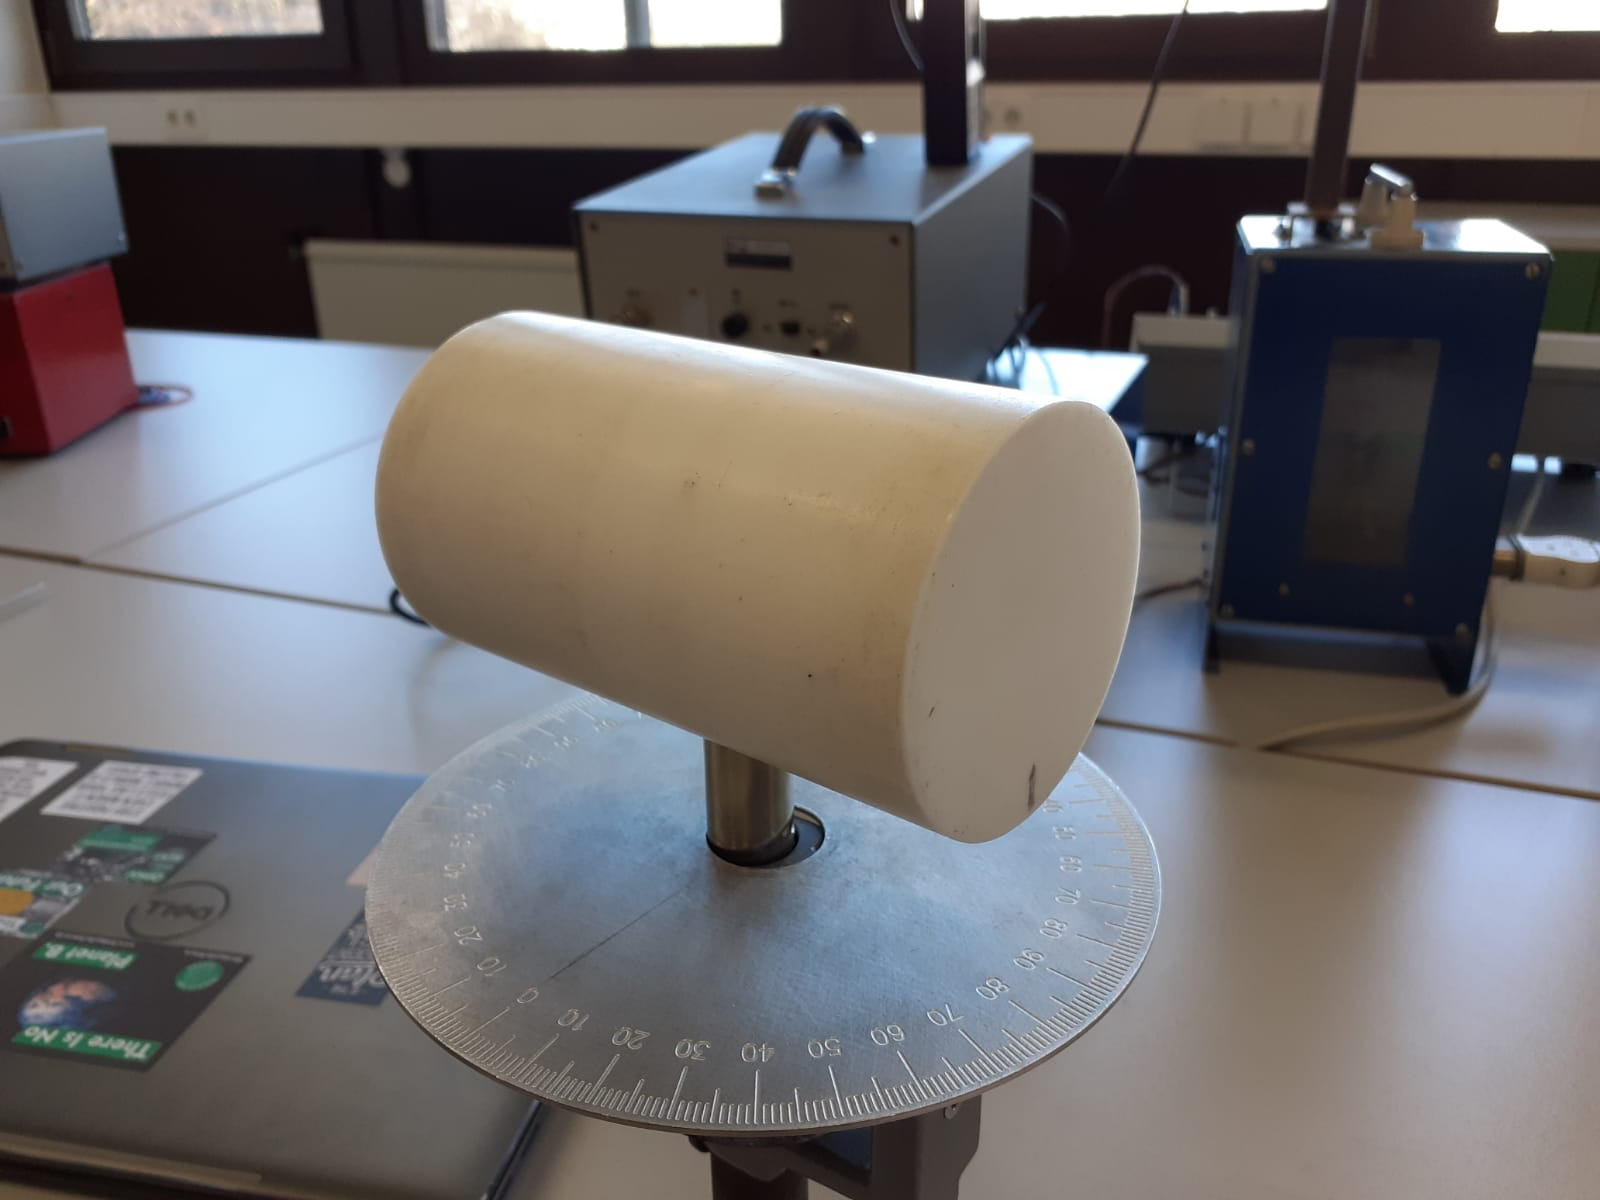
\includegraphics[height=5cm]{plots/Zyl_big.jpeg}
        \caption{Der große Zylinder.}
        \label{fig:grZyl}
    \end{subfigure}
    \begin{subfigure}{0.48\textwidth}
        \centering
        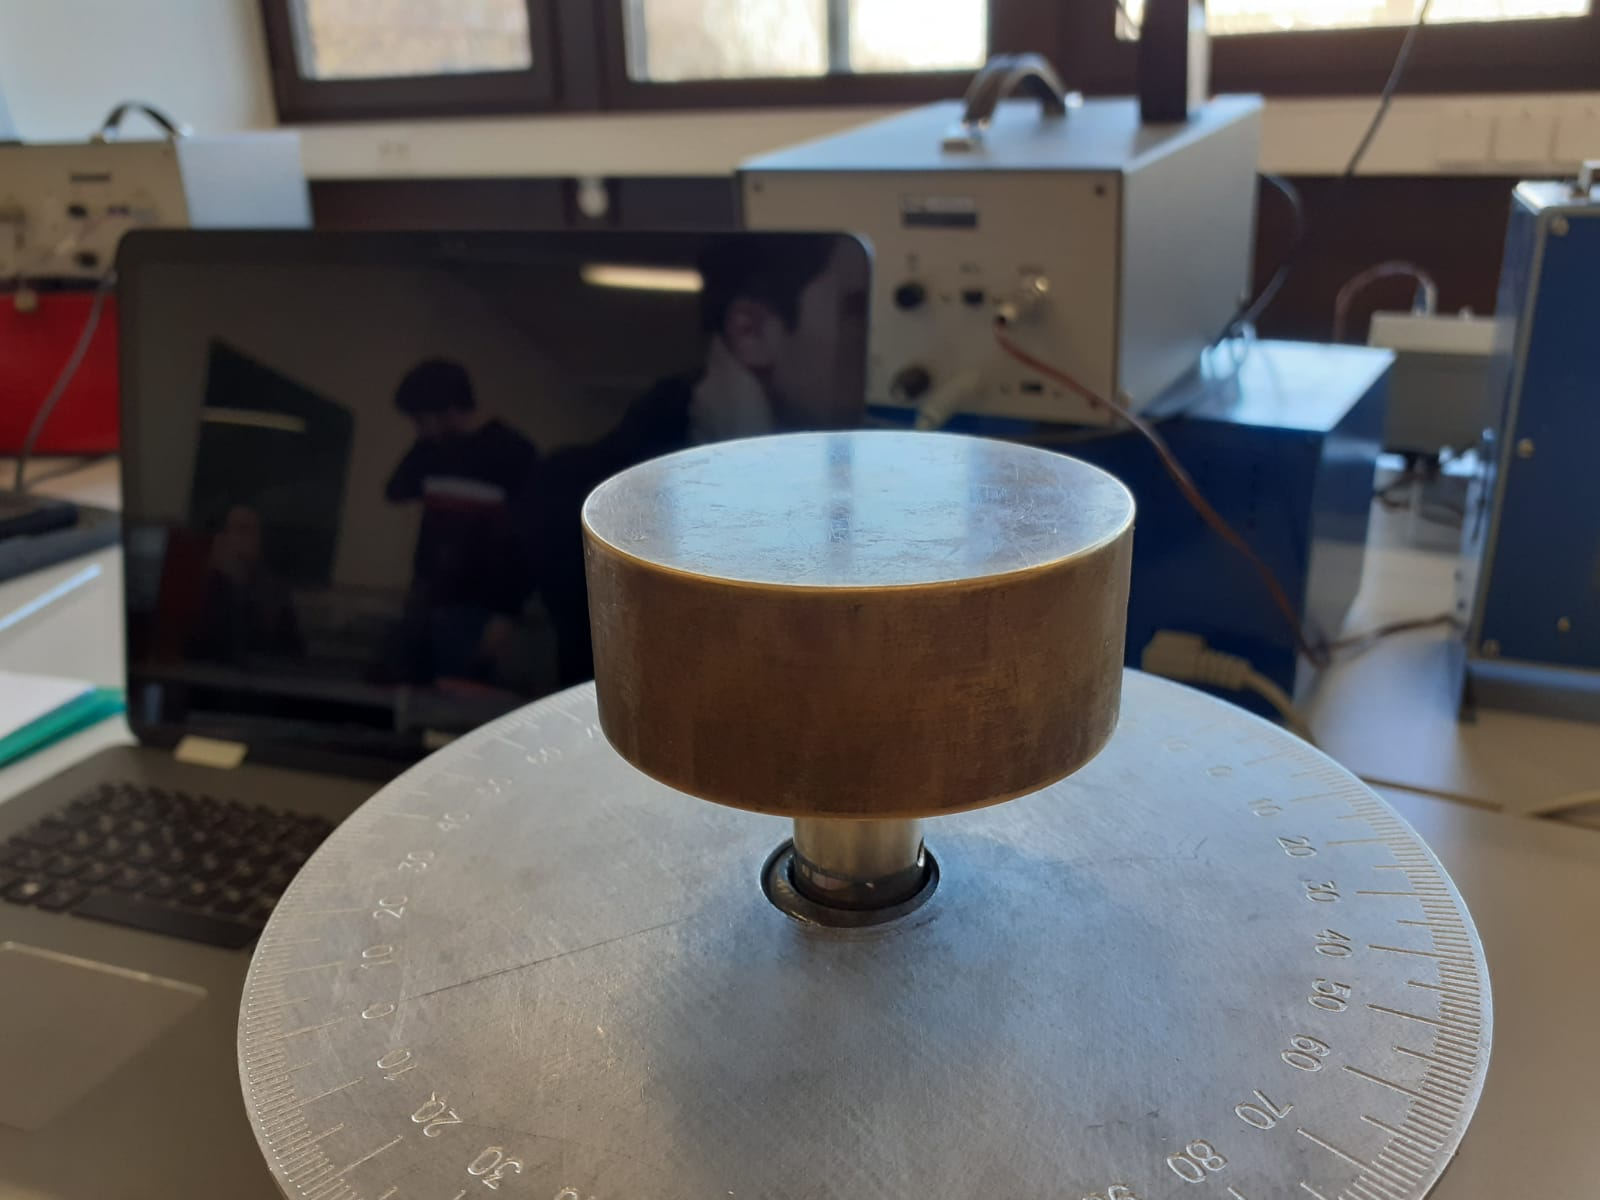
\includegraphics[height=5cm]{plots/Zyl_small.jpeg}
        \caption{Der kleine Zylinder.}
        \label{fig:klZyl}
    \end{subfigure}
    \caption{Die verwendeten Zylinder und ihre Drehachsen im Experiment.}
    \label{fig:Zyl}
\end{figure}

\begin{figure}
    \centering
    \begin{subfigure}{0.48\textwidth}
        \centering
        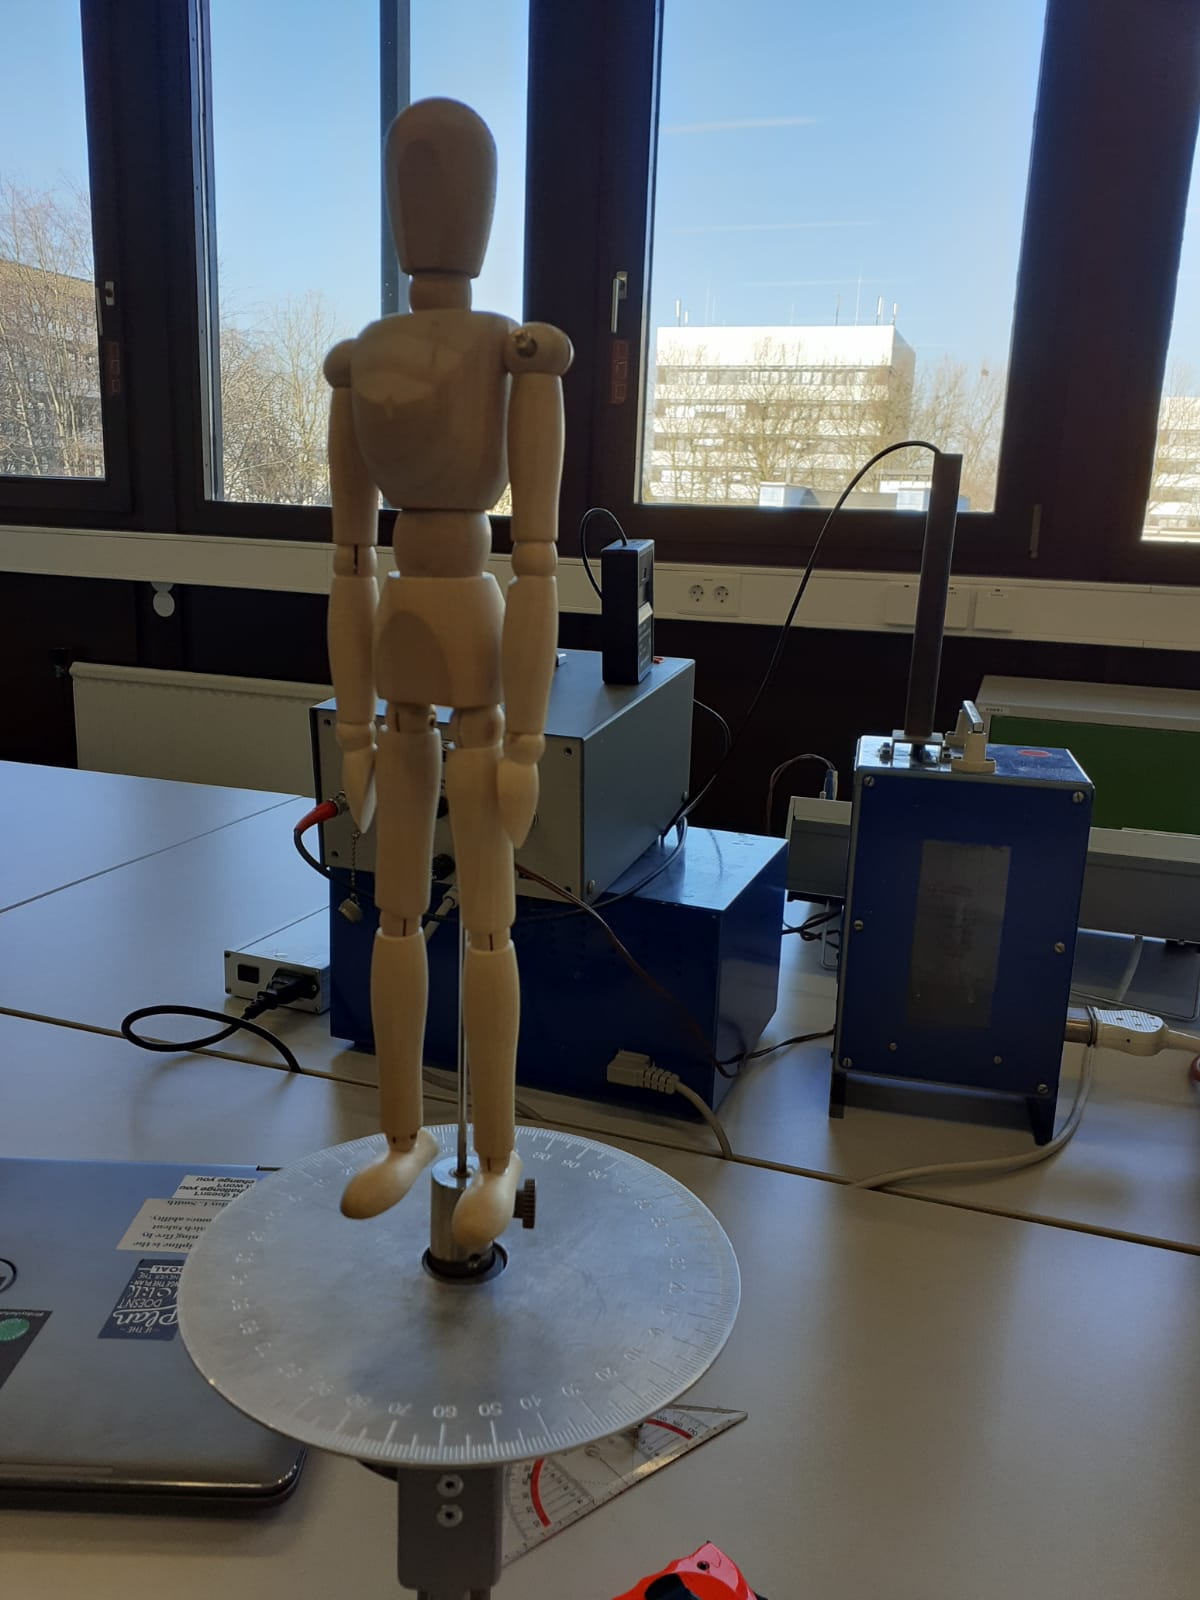
\includegraphics[height=5cm]{plots/figur1.jpeg}
        \caption{Pose 1.}
        \label{fig:pos1}
    \end{subfigure}
    \begin{subfigure}{0.48\textwidth}
        \centering
        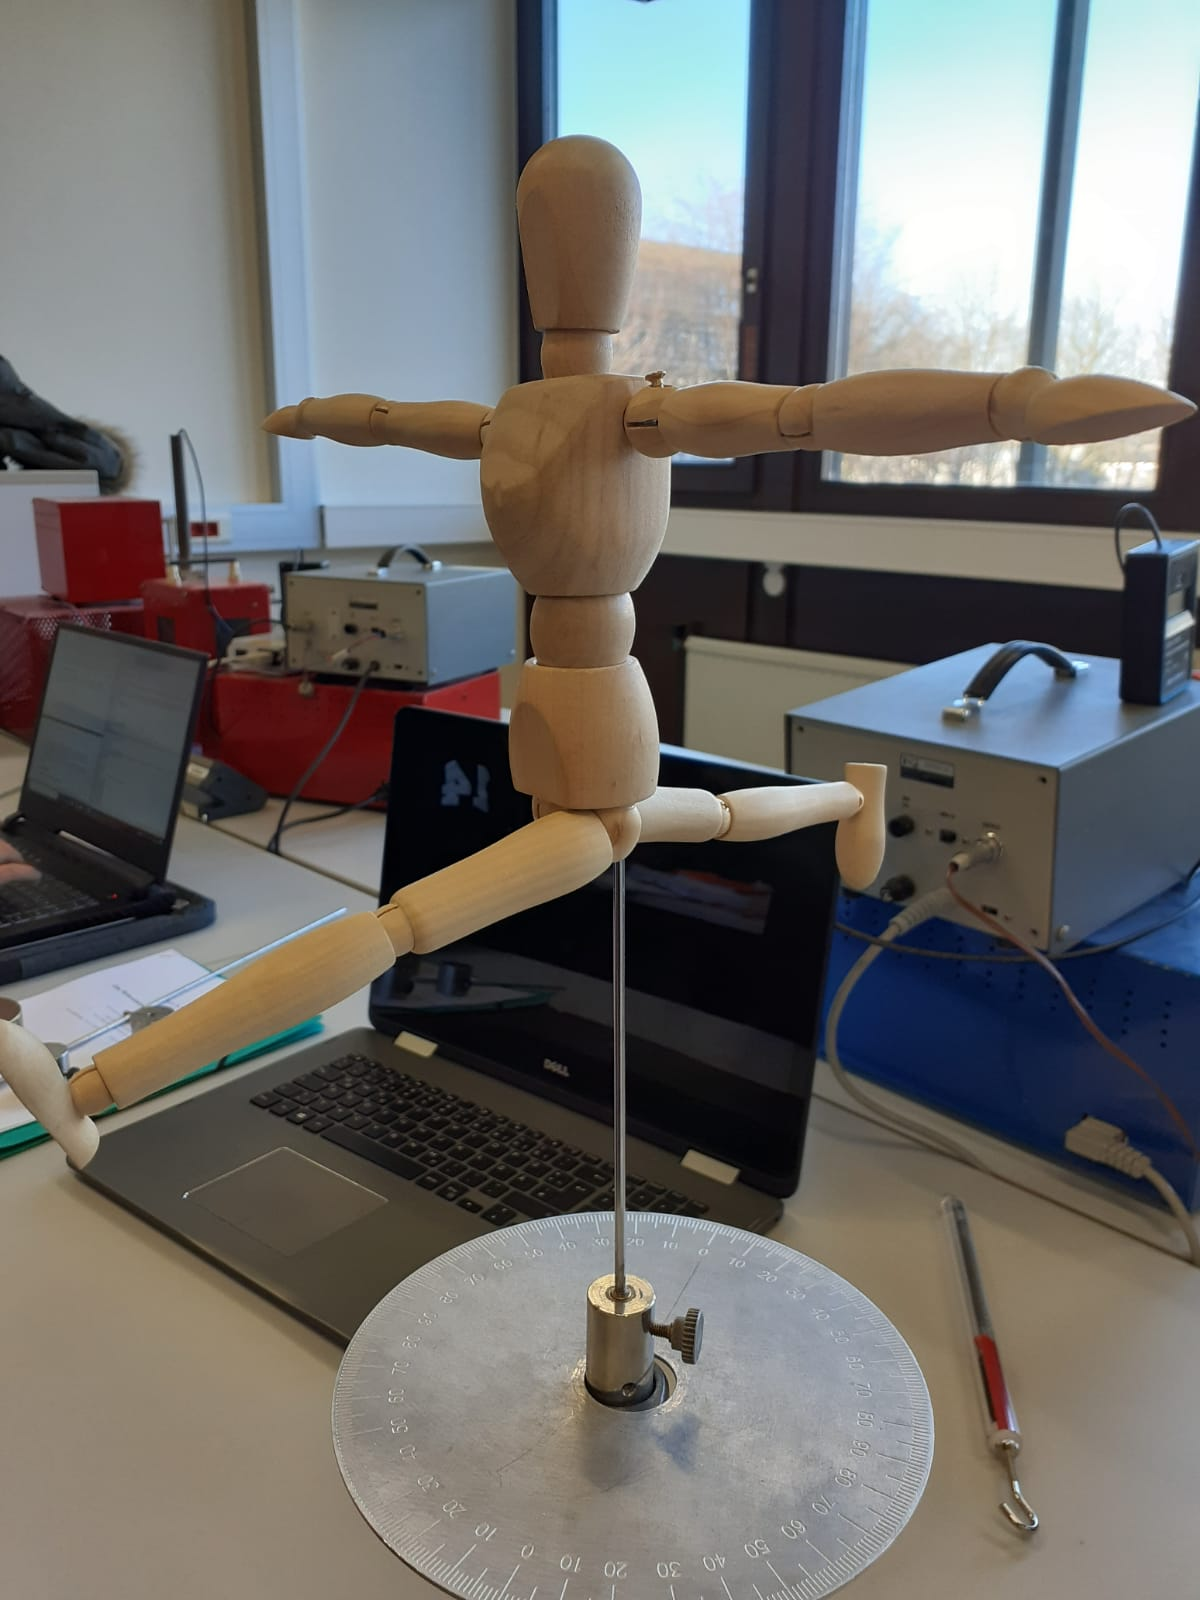
\includegraphics[height=5cm]{plots/figur2.jpeg}
        \caption{Pose 2.}
        \label{fig:pos2}
    \end{subfigure}
    \caption{Die Holzpuppe in zwei verschiedenen Stellungen.}
    \label{fig:puppe}
\end{figure}

\begin{table}
    \centering
    \caption{Messwerte aller Schwingungsdauern.}
    \label{tab:messSchwing}
    \begin{tabular}{c c c c}
        \toprule
        {$T_\text{Zyl,groß}\:/\:\si{\second}$} & {$T_\text{Zyl,klein}\:/\:\si{\second}$} & {$T_\text{Pose1}\:/\:\si{\second}$} & {$T_\text{Pose2}\:/\:\si{\second}$} \\
        \midrule
        1.08 & 2.31 & 0.38 & 0.92 \\
        1.27 & 2.23 & 0.41 & 0.89 \\
        1.13 & 2.17 & 0.43 & 0.94 \\
        1.18 & 2.30 & 0.39 & 0.91 \\
        1.16 & 2.26 & 0.41 & 0.91 \\
        \bottomrule
    \end{tabular}
\end{table}

\begin{table}
    \centering
    \caption{Messunsicherheiten aller Schwingungsdauern.}
    \label{tab:mittelSchwing}
    \begin{tabular}{l c}
        \toprule
        & {T$\:/\:\si{\second}$} \\     % werden Messgrößen kursiv geschrieben? (hier das T)
        \midrule
        Zylinder$_\text{gross}$  & $\SI{2.25(5)}{}$ \\
        Zylinder$_\text{klein}$  & $\SI{1.16(6)}{}$ \\
        Holzfigur Pose 1  & $\SI{0.40(2)}{}$ \\
        Holzfigur Pose 2  & $\SI{0.91(2)}{}$ \\
        \bottomrule
    \end{tabular}
\end{table}

\FloatBarrier
\subsubsection{Der kleine Zylinder}

\begin{table}
    \centering
    \caption{Maße des kleinen Zylinders und der zugehörigen Halterung.}
    \label{tab:kleZyl}
    \begin{tabular}{c c}
        \toprule
        \multicolumn{2}{c}{Zylinder} \\
        \midrule
        $m$ & \SI{1119.4}{\gram} \\
        $h$ & \SI{3.0}{\centi\meter} \\
        $d$ & \SI{7.45}{\centi\meter} \\
        \bottomrule
    \end{tabular}
    \qquad \qquad 
    \begin{tabular}{c c}
        \toprule
        \multicolumn{2}{c}{Halterung}\\
        \midrule
        $h$ & \SI{1.8}{\centi\meter} \\
        $d$ & \SI{0.6}{\centi\meter} \\
        \bottomrule
            \\
    \end{tabular}
\end{table}

Das erwartete Trägheitsmoment anhand der geometrischen Abmessungen ist 
\begin{gather}
    m_\text{ges}=\SI{1119.4}{\gram}\:, \qquad 
    m_\text{Zyl}=m_\text{ges}\frac{d_\text{Zyl}^2h_\text{Zyl}}{d_\text{Zyl}^2h_\text{Zyl}+d_\text{Halt}^2h_\text{Halt}}=\SI{1115.1}{\gram} \\
    m_\text{Halt} = m_\text{ges}-m_\text{Zyl}=\SI{4.3}{\gram} \\
    I_\text{kl,geo}=\frac{1}{2}m_\text{Zyl}\frac{d_\text{Zyl}^2}{4}+\frac{1}{2}m_\text{Halt}\frac{d_\text{Halt}^2}{4}=\SI{7.74}{\kilo\gram\centi\meter\squared}\:.
\end{gather}

Wird hingegen die gemittelte Periode und die Winkelrichtgröße inklusive der Messfehler verwendet, um über 
\begin{equation}
    T=2\symup{\pi}\sqrt{\frac{I}{D}}
\end{equation}
das Trägheitsmoment zu berechnen, ergibt sich 
\begin{equation}
    I_\text{kl,T}=T^2\frac{D}{4\symup{\pi}^2}=\SI{6.44(55)}{\kilo\gram\centi\meter\squared}\:.
\end{equation}

\FloatBarrier
\subsubsection{Der große Zylinder}

Dasselbe Verfahren wird nun für den großen Zylinder angewendet, mit dem Unterschied, dass die Drehachse hier senkrecht zur 
Symmetrieachse des Zylinders steht und deshalb eine etwas abgewandelte, in der Theorie erläuterte Formel verwendet wird. 

\begin{table}
    \centering
    \caption{Maße des großen Zylinders und der zugehörigen Halterung.}
    \label{tab:groZyl}
    \begin{tabular}{c c}
        \toprule
        \multicolumn{2}{c}{Zylinder}\\
        \midrule
        $m$ & \SI{1525.6}{\gram} \\
        $h$ & \SI{13.95}{\centi\meter} \\
        $d$ & \SI{7.95}{\centi\meter} \\
        \bottomrule
    \end{tabular}
    \qquad \qquad 
    \begin{tabular}{c c}
        \toprule
        \multicolumn{2}{c}{Halterung}\\
        \midrule
        $h$ & \SI{1.4}{\centi\meter} \\
        $d$ & \SI{0.55}{\centi\meter} \\ 
        \bottomrule
            \\
    \end{tabular}
\end{table}

\begin{gather}
    m_\text{ges}=\SI{1525.6}{\gram}\:, \qquad 
    m_\text{Zyl}=m_\text{ges}\frac{d_\text{Zyl}^2h_\text{Zyl}}{d_\text{Zyl}^2h_\text{Zyl}+d_\text{Halt}^2h_\text{Halt}}=\SI{1524.9}{\gram} \\
    m_\text{Halt} = m_\text{ges}-m_\text{Zyl}=\SI{0.7}{\gram} \\
    I_\text{gr,geo}=m_\text{Zyl} \Bigl( \frac{d_\text{Zyl}^2}{16} + \frac{h_\text{Zyl}^2}{12} \Bigr) 
        +\frac{1}{2}m_\text{Halt}\frac{d_\text{Halt}^2}{4}=\SI{30.75}{\kilo\gram\centi\meter\squared}\:.
\end{gather}

\begin{equation}
    I_\text{gr,T}=T^2\frac{D}{4\symup{\pi}^2}=\SI{24.24\pm2.32}{\kilo\gram\centi\meter\squared}\:.
\end{equation}

